%!TEX root = report.tex

\chapter{Déploiement et Tests}

\section{Introduction du Chapitre}

Ce chapitre porte sur les méthodes utilisées pour déployer notre application dans l'environnement de test ainsi que les techniques de teste utilisés.

\section{Déploiement}

Pour transférer notre application sur le terminal \android{} on utilise un outil fourni dans l'\gls{sdk}: \gls{adb}.

\gls{adb}\cite{tools:adb} est un outil versatile en ligne de commande qui nous permet de communiquer avec une instance d'un émulateur ou un équipement \android{} connecté. C'est un programme de type client-serveur qui inclue 3 composants:

\begin{itemize}

\item Un client, qui tourne sur notre machine de développement. On peut invoquer
un client depuis une invite de commande par l’envoi d'une commande \gls{adb}.
D'autre outils \android{} comme le plugin \gls{adt} et le \gls{ddms} crée eux
aussi des clients \gls{adb}.

\item Un serveur, qui tourne comme un processus de fond dans notre machine de
développement. Le serveur gère les communications entre le client et le démon
\gls{adb} qui tourne dans une instance d'un émulateur ou un terminal.

\item Un démon, qui tourne comme un processus de fond dans chaque instance de l’émulateur ou terminal.

\end{itemize}

On peut retrouver l'outil \gls{adb} dans le dossier $<sdk>/platform-tools/$.

On peut utiliser \gls{adb} pour copier une application depuis notre machine de développement et l'installer dans une instance d'un émulateur ou un terminal, pour cela on utilise la commande \cmd{install}. Cette commande exige comme paramètre le chemin du fichier .apk que nous voulons installer.


\begin{lstlisting}[language=bash, label=lst:adb_install, caption=Exemple d'utilisation du commande adb install]

$adb install ~/tunavmedi.apk

\end{lstlisting}

Notant qu'avec Eclipse équipé du plugin \gls{adt} on n'a pas besoin d'utiliser
\gls{adb} directement pour installer notre application sur l'émulateur ou le
terminal. Le plugin \gls{adt} s'occupe du packaging et de l'installation de
l'application pour nous.


Pour désinstaller une application on utilise le \en{Package Manager}. On peut
envoyer des commandes avec le \en{Package Manager} pour effectuer des actions et
des opérations de recherches sur les paquetages des applications installées dans
l'émulateur ou le terminal. Listing \ref{lst:adb_pm} présente la syntaxe
générale de l'outil tandis que le listing \ref{lst:adb_uninstall} présente la
syntaxe utilisé pour désinstaller notre application.


\begin{lstlisting}[language=bash, label=lst:adb_pm, caption=Syntaxe générale de l'utilisation du Package Manager]

$pm <command>

\end{lstlisting}

\begin{lstlisting}[language=bash, label=lst:adb_uninstall, caption=Exemple de désinstallation]

$adb shell pm uninstall com.tunav.tunavmedi

\end{lstlisting}

\subsection{Détecteur de bugs: Android Lint}

\begin{figure}[H]
\center
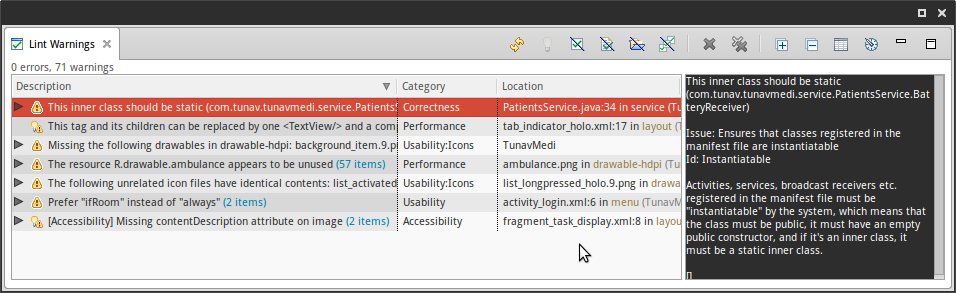
\includegraphics[width=0.9\textwidth]{lint}
\caption{Problèmes potentiels dans notre application détectés par Android Lint.}
\label{fig:lint}
\end{figure}

\android{} \en{Lint} (figure \ref{fig:lint}) est un outil introduit dans la version 16 de \gls{adt} qui scanne les code sources des projets \android{} afin d'y détecter des mal-fonctions potentielles.

Quelques exemples de types d'erreurs que cet outil permet de détecter sont:

\begin{itemize}

\item Translations manquantes ou inutilisés.

\item Les problèmes de performance dans les \dev{Layout}.

\item Ressources inutilisées

\item Tableau de taille inconsistante (dans le cas ou le tableau est défini dans des configurations différentes).

\item Problème d'accessibilités et d'internationalisation.

\item Problème d'icônes (Tailles manquantes, doubles, fausse résolution).

\item Problème d'usabilité .

\item Erreurs dans le \dev{Manifest}.

\end{itemize}

Dans Eclipse, \android{} Lint est disponible à travers le menu Window $\rightarrow$ Show View $\rightarrow$ Other... puis on sélectionne \en{Lint Warning} dans la fenêtre qui s'affiche (figure \ref{fig:lint_eclipse}).

\begin{figure}
\center
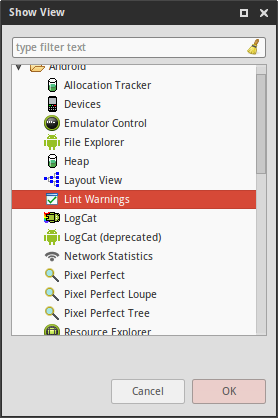
\includegraphics[width=0.4\textwidth]{lint_eclipse}
\caption{Accéder à Android Lint dans Eclipse}
\label{fig:lint_eclipse}
\end{figure}

\section[UI/Application Exerciser Monkey]{\en{UI/Application Exerciser Monkey}}

\en{Monkey} \cite{tools:monkey} est un programme qui tourne sur notre émulateur ou terminal \android{} et qui génère des flux pseudo-aléatoire d’événements utilisateur comme par exemple les clics, les touchés, les gestes, ou encore un nombre d’événements de niveau système. On peut utilisés \en{Monkey} pour effectuer des tests de stresse sur notre application dans une manière aléatoire et répétitive.

L'annexe \ref{chptr:monkey} montre un exemple de test effectué avec l'outil \en{Monkey} sur notre application.